% %# -*- coding: utf-8-unix -*-
% % !TEX program = xelatex
% % !TEX root = ../thesis.tex
% % !TEX encoding = UTF-8 Unicode
% \chapter{常见问题}
% \label{chap:faq}

% {\bfseries{}Q:我是否能够自由使用这份模板?}

% A:这份模板以Apache License 2.0开源许可证发布,请遵循许可证规范。

% {\bfseries{}Q:我的论文是Word排版的,学校图书馆是不是只收 \LaTeX 排版的论文?}

% A:当然不是,Word版论文肯定收。

% {\bfseries{}Q:我的论文是 \LaTeX 排版的,学校图书馆是不是只收Word排版的论文?}

% A:当然不是,PDF版的电子论文是可以上交的。是否要交Word版就看你导师的喜好了。

% {\bfseries{}Q:为什么屏幕上显示的左右页边距不一样?}

% A:模板默认是双面打印,迎面页和背面页的页边距是要交换的,多出来的那一部分是留作装订的。

% {\bfseries{}Q:为什么在参考文献中会有“//”符号?}

% A:那就是国标GBT7714参考文献风格规定的。但可以使用 gbpunctin=false 选项将其还原成 in:,进一步可以在导言区加入\verb+\DefineBibliographyStrings{english}{in={}}+将其去掉。

% {\bfseries{}Q:为什么参考文献中会有[s.n.],[S.l], [EB/OL]等符号?}

% A: 那也是国标GBT7714参考文献风格定义的。[s.n.]表示出版者不祥,[S.l]表示出版地不祥,[EB/OL]表示引用的参考文献类型为在线电子文档。但可以使用gbpub=false 选项将其缺省补充的出版项[s.n.]等去掉。也可以使用选项 gbtype=false 将参考文献类型标识去掉。

% {\bfseries{}Q:如何获得帮助和反馈意见?}

% A:你可以通过\href{https://github.com/sjtug/SJTUThesis/issues}{在github上开issue}
% 、在\href{https://bbs.sjtu.edu.cn/bbsdoc?board=TeX_LaTeX}{水源LaTeX版}发帖反映你使用过程中遇到的问题。

% {\bfseries{}Q:使用文本编辑器查看tex文件时遇到乱码?}

% A:请确保你的文本编辑器使用UTF-8编码打开了tex源文件。

% {\bfseries{}Q:在CTeX编译模板遇到“rsfs10.tfm already exists”的错误提示?}

% A:请删除\verb+X:\CTEX\UserData\fonts\tfm\public\rsfs+下的文件再重新编译。问题讨论见\href{https://bbs.sjtu.edu.cn/bbstcon,board,TeX_LaTeX,reid,1352982719.html}{水源2023号帖}。

% {\bfseries{}Q:升级了TeXLive 2012,编译后的文档出现“minus”等字样?}

% A:这是xltxtra和fontspec宏包导致的问题。学位论文模板从0.5起使用metatlog宏包代替xltxtra生成 \XeTeX 标志,解决了这个问题。

% {\bfseries{}Q:为什么在bib中加入的参考文献,没有在参考文献列表中出现?}

% A: bib中的参考文献条目,常通过\verb+\cite+或\verb+\parencite+或\verb+\supercite+或\verb+\textcite+等命令在正文中引用进而加入到参考文献列表中。当需要将参考文献条目加入到文献表中但又不引用可以使用\verb+\nocite+命令,当nocite参数为*时则引入bib中的所有文献。
% %\verb+\upcite+ 是哪个宏包的?之前没有见过

% {\bfseries{}Q:我可以使用Sublime Text编写学位论文吗?}

% A: 可以。首先\href{https://www.sublimetext.com/}{下载}并安装Sublime Text,然后安装
% \href{https://packagecontrol.io/installation}{Package Control},
% 之后按\verb|ctrl+shift+p|或者\verb|cmd+shift+p|调出命令窗口,
% 输入\verb|install|,选择\textit{Package Control: Install Package},按回车,
% 稍等片刻,等待索引载入后会弹出选项框,输入\verb|LaTeXTools|并回车,即可成功安装插件。
% 之后只需要打开\verb|.tex|文件,按\verb|ctrl+b|或者\verb|cmd+b|即可编译,
% 如有错误,双击错误信息可以跳转到出错的行。

% {\bfseries{}Q:在macTex中,为什么pdf图片无法插入?}

% A:如果报错是“pdf: image inclusion failed for "./figure/chap2/sjtulogo.pdf".”,则采取以下步骤

% \begin{lstlisting}[basicstyle=\small\ttfamily, caption={编译模板}, numbers=none]
% brew install xpdf
% wget http://mirrors.ctan.org/support/epstopdf.zip
% unzip epstopdf.zip
% cp epstopdf/epstopdf.pl /usr/local/bin/
% cd figure/chap2
% pdftops sjtulogo.pdf
% epstopdf sjtulogo.ps
% pdfcrop sjtulogo.pdf
% mv sjtulogo.pdf backup.pdf
% mv sjtulogo-crop.pdf sjtulogo.pdf
% \end{lstlisting}

% {\bfseries{}Q:为什么维普等查重系统无法识别此模板生成的 pdf 内所有的中文?}

% A: 中文无法识别的情况多半是由于使用了 ShareLaTeX 的原因,请尝试使用 TexStudio 等软件在本地进行编译。
% 如果使用 TeXstudio 请在 Preferences-Build 中将 Default Compiler 和 Default Bibliography Tool 分别改为 XeLaTeX 和 Biber。

% {\bfseries{}Q:如何向你致谢?}

% A: 烦请在模板的\href{https://github.com/sjtug/SJTUThesis}{github主页}点击“Star”,我想粗略统计一下使用学位论文模板的人数,谢谢大家。非常欢迎大家向项目贡献代码。


\chapter{基于映射的INL2SQL生成}
\label{chap:interaction}
本章研究交互式自然语言接口生成SQL 查询语句(INL2SQL)的技术与方法。

\section{研究问题}

一直以来,自然语言接口是人机交互领域的终极追求,也是人机交互、机器学习领域专家孜孜不倦钻研探索的热门问题。
交互式自然语言接口生成SQL查询语句(INL2SQL)的关键问题就是怎样使得系统能在与用户的多轮交互之下理解到用户的查询意图,并结合数据库模式直接生成符合查询意图的SQL语句。
其主要过程为:用户首先输入自然语言查询语句以及给出对应的数据库模式,系统接收到输入后理解输入,并和用户产生多轮交互,在交互完成并确认输出后将对应的SQL查询语句及执行结果输出。
% 因此,本章将对从自然语言生成SQL语句的技术和模型进行探究,尝试寻找一种解决方案,能提供自然语言接口给非技术用户,让用户通过以自然语言表达的查询意图,得到目标SQL语句。

\begin{figure}[!htp]
  \centering
  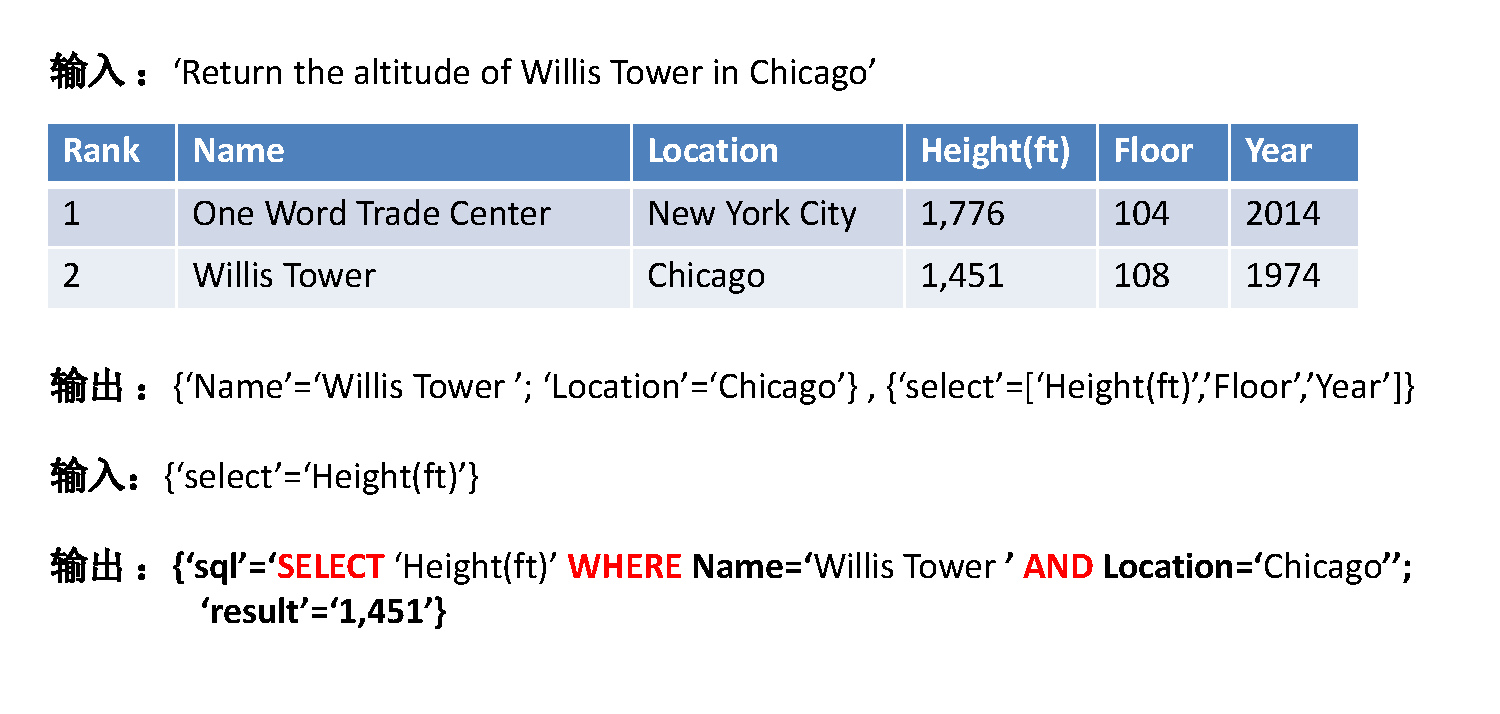
\includegraphics[width=15cm]{example/nli.pdf}
  \bicaption[INL2SQL生成示例]
    {INL2SQL生成示例}
    {An Example of Interactive Nature Language to SQL Query Statement}
  \label{fig:NLI}
\end{figure}

图\ref{fig:NLI}中给出了INL2SQL生成的一个示例。
用户首先输入自然语言查询语句“Return the altitude of Willis Tower in Chicago”。
系统根据给定的数据库模式,判断出两个有效过滤条件即‘Name’=‘Willis Tower ’和‘Location’=‘Chicago’但不确认聚合函数是否为‘SELECT’及其对象是否为‘Height(ft)’。系统返回一个包含{‘Name’=‘Willis Tower ’; ‘Location’=‘Chicago’}和{‘select’=[‘Height(ft)’,’Floor’,’Year’]}的交互项。
其中{‘Name’=‘Willis Tower ’; ‘Location’=‘Chicago’}表示为已经确认的信息,{‘select’=[‘Height(ft)’,’Floor’,’Year’]}为json格式表示需要用户在‘Height(ft)’,’Floor’,’Year’中做出选择。
用户接受到交互信息后进行选择并发送包含{‘select’=‘Height(ft)’}的json数据。
最后,系统在多轮交互并确认输出有效后将对应的SQL查询语句‘SELECT ‘Height(ft)’ WHERE Name=‘Willis Tower’ AND Location=‘Chicago’及执行结果‘1,451’输出。
% 自然语言理解存在许多难题,如歧义、语序,或者存在复杂的依赖结构等等,要完全基于自然语言理解来进行SQL生成是很困难的,效果可能会不尽如人意。
% 所以,受到人机交互思想的启发,本文将使用自然语言理解与人机交互相结合的方式,来进行从自然语言到目标SQL语句的转化。
% 对于自然语言意图,先对自然语言进行初步解析和理解,并在其中插入人机交互机制,让用户来引导生成的过程,指导自然语言理解,纠正机器理解过程中出现的错误、歧义、含糊不清的问题,从而提升整体的准确性。



\section{相关工作}
在软件产品的开发与使用过程中,非专家用户常常会在指定的关系型数据库上使用关键字搜索\cite{bhalotia2002keyword,yu2010keyword,agrawal2002dbxplorer,hristidis2002discover}来进行实时的查询。
所以近年以来,有很多的研究人员对关键字搜索领域进行研究\cite{tata2008sqak,simitsis2008precis,ganti2010keyword++,blunschi2012soda,bergamaschi2013quest}。
关键字搜索的目的不是通过输入的关键字的集合来找到与这些关键字相关联的数据,而是通过这些关键字来推测并解析出其背后想要表达的查询意图及对应的自然语言。
在这些研究中,有的方法通过聚合函数\cite{tata2008sqak}、布尔运算符\cite{simitsis2008precis}、查询语句片段\cite{blunschi2012soda}等方式对关键字进行拓展。
现在看来,这些研究内容是解决自然语言查询这一挑战的奠基者。
本文所提出的解决方案能够支持更加丰富的查询,使得用户可以使用语义更加复杂的语句进行查询。

数据库的自然语言接口(NLIDB)已经被研究人员研究了很长的时间\cite{Androutsopoulos1995Natural}。
早期的NLIDB需要依靠为每个数据库单独定制的手工语法来进行查询,这些手工语法的拓展性很差,很难在其他数据库中进行使用。
相比之下,本文所提出的解决方案以生成SQL查询语句作为目的,具有很好的通用性,可以被移植到其他的数据库上使用。
 
NLIDB在使用上最大的问题在于其所依赖的信息很有限,正常的自然语言往往是没有一个固定的格式和语义\cite{popescu2003towards}。
这也就导致了NLIDB无法准确地推断用户输入的查询意图。
为了解决可靠性的问题,Popescu等人\cite{popescu2003towards,popescu2004modern}采用了PRECISE方法,将输入的自然语言查询划分为语义更加容易被解析的查询片段,并将这些查询片段更为精确地转换为SQL查询语句。
但是,PRECISE无法处理那些语义不确切或者难以处理的自然语言查询。
相比而言,本文提出的解决方案通过与用户的多轮交互,可以较好地解决语义不明确的问题。

也有很多文献\cite{Androutsopoulos1995Natural,kuepper1993nauda,li2005nalix}提出过交互式NLIDB的想法,早期交互式NLIDB\cite{Androutsopoulos1995Natural,kuepper1993nauda}主要目标在于从查询生成对应的结果。
而NaLIX\cite{li2005nalix}则更进一步,当用户的查询超出模型的语义理解能力的范围之外时会把相应的重构查询的建议返回给用户,这种策略会大大减少用户在使用时对其查询进行重构的负担。
然而,NaLIX对输入的查询超过模型的语义理解能力的处理方式不太正确。
而在本文提出的解决方案中,对于给定的自然语言查询语句,系统会与用户多轮交互并向用户解释意图解析与SQL生成的过程,从而对查询进行重构,解决歧义问题。
所以,在与用户的多轮反馈与交互下,用户可以输入较为复杂的查询,其生成的SQL查询语句可以包含多级聚合操作、嵌套以及各种类型的连接操作等。

\section{解决方案}
\begin{figure}[!htp]
    \centering
    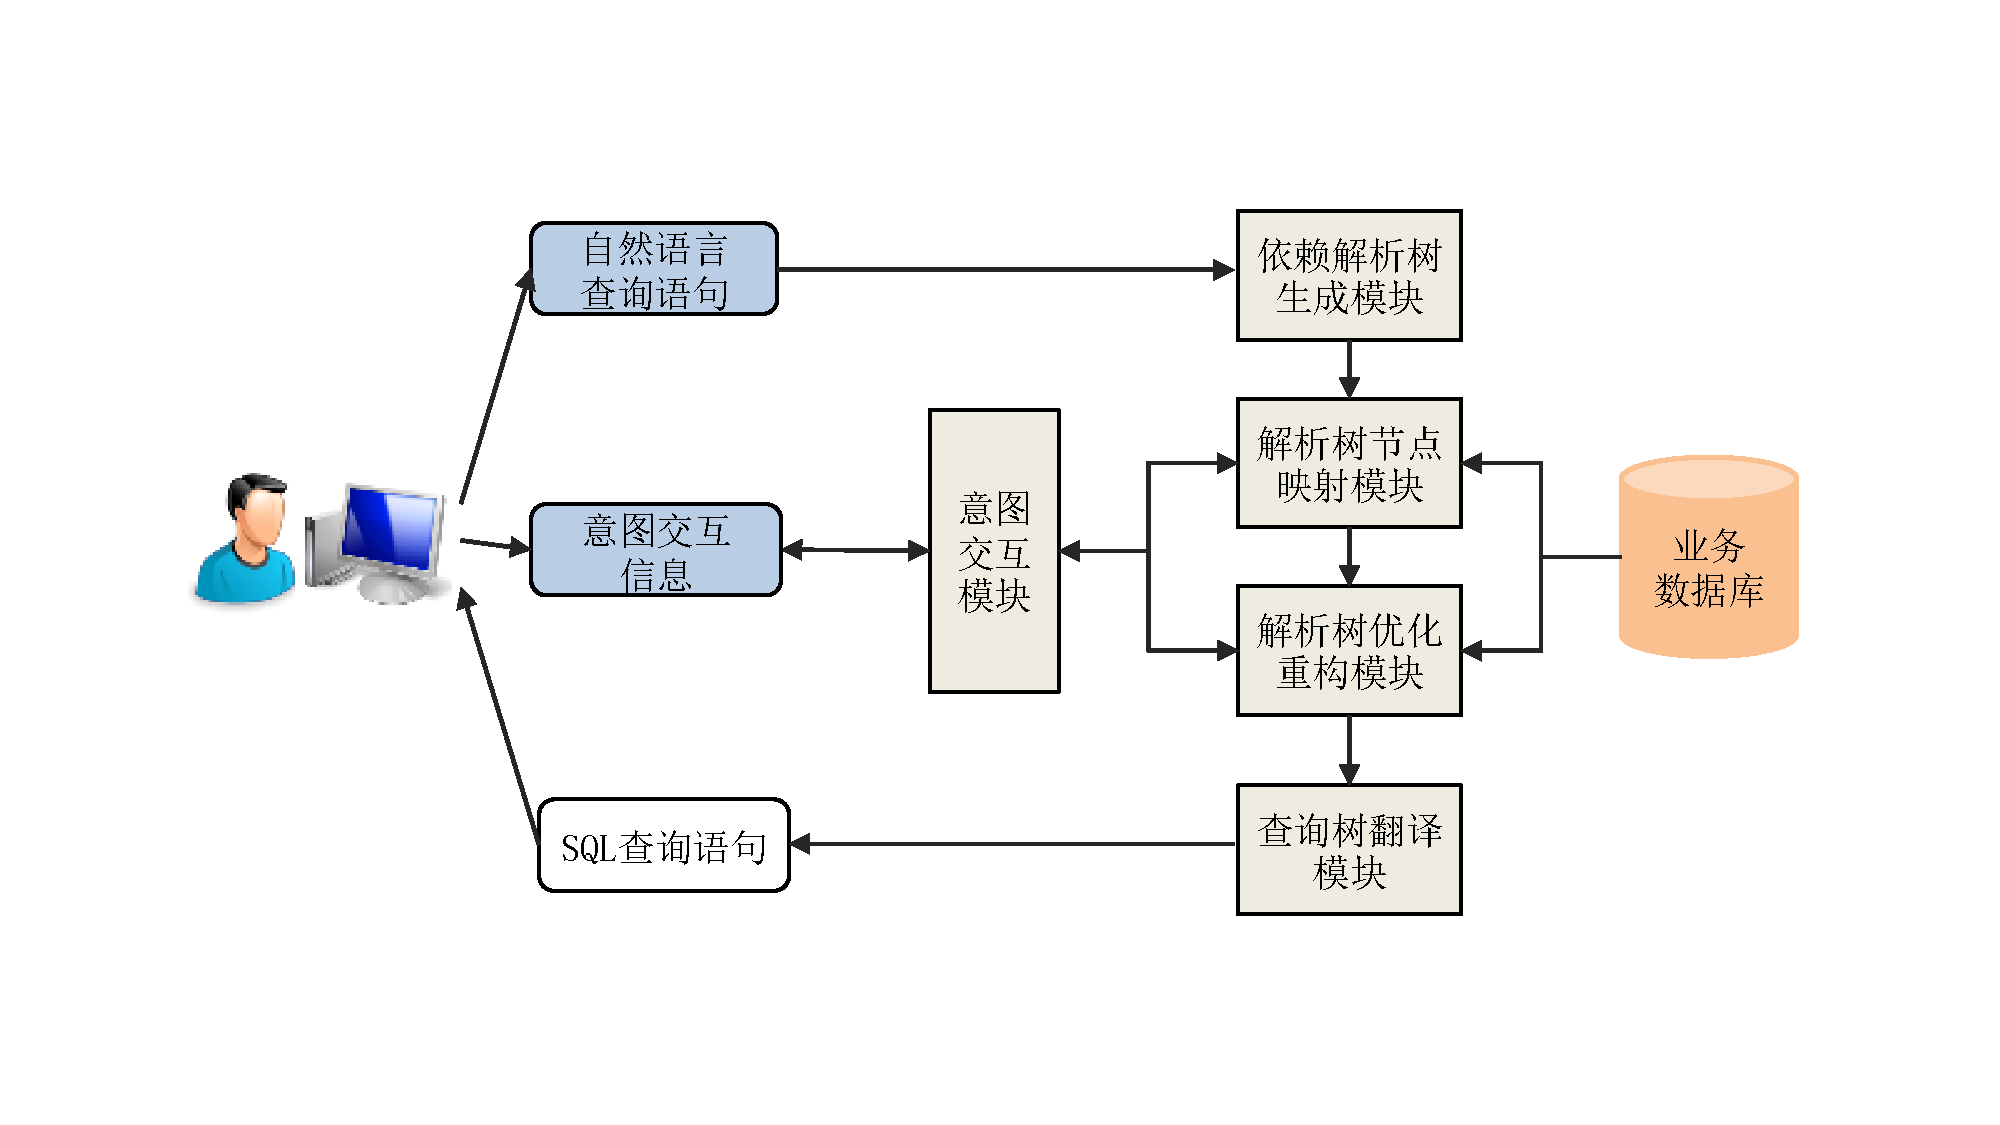
\includegraphics[width=15cm]{example/NLIapproach.pdf}
    \bicaption[基于映射的INL2SQL生成的总体方案]
      {基于映射的INL2SQL生成的解决方案}
      {Approach on Interactive Nature Language to SQL Query Statement through Mapping}
    \label{fig:NLIapproach}
  \end{figure}

图\ref{fig:NLIapproach}是基于映射的INL2SQL生成的解决方案,它包含依赖解析树生成、解析树节点映射、解析树优化重构、查询树翻译、意图交互五个模块:
\begin{enumerate}
    % \item 用户接口:用户与系统进行交互的接口,包括输入自然语言、返回SQL语句、解析过程中的交互等等。
    \item 依赖解析树生成:将用户输入的、以自然语言表示的查询意图,应用自然语言理解技术,转化为依赖解析树,即将词语进行词性标注,识别出词语之间的关系,并将其组织成一个树状结构。详见\ref{nli:yljxssc}节。
    \item 解析树节点映射:根据解析树节点对应的词语和数据库模式、SQL语法等信息,将解析树节点映射为SQL语法组件。
在这个过程中,如果节点的映射有多个候选答案,意图交互模块会发起与用户的交互,将多个候选映射展示给用户,让用户来进行选择。详见\ref{nli:jxsjdys}节。
    \item 意图交互:管理解析过程与用户的交互,在适当的时候与用户进行交互,让用户对解析过程进行反馈与指导。
    \item 解析树优化重构:节点映射完毕后,解析树节点经过系统匹配和用户指导后,得到了比较准确的结果,但解析树的结构仍是最初由依赖解析树生成得到的结构,这一原始结构的准确度并不高,受限于自然语言的复杂性和省略性,可能会有错误关系、缺失关系、缺失节点等等。
因此系统将根据算法和规则,修正错误关系,补全缺失节点和缺失关系,得到较为准确的解析树,称为查询树。详见\ref{nli:jxsyhcg}节。
    \item 查询树翻译:解析树的结构已经符合SQL语法,节点映射结果也对应于真实的SQL语法、数据库模式或数据,可以很自然地将树状结构翻译为SQL语句,最后将SQL语句(及查询结果)返回给用户。详见\ref{nli:cxsfy}节。
\end{enumerate}

\begin{figure}[!htp]
  \centering
  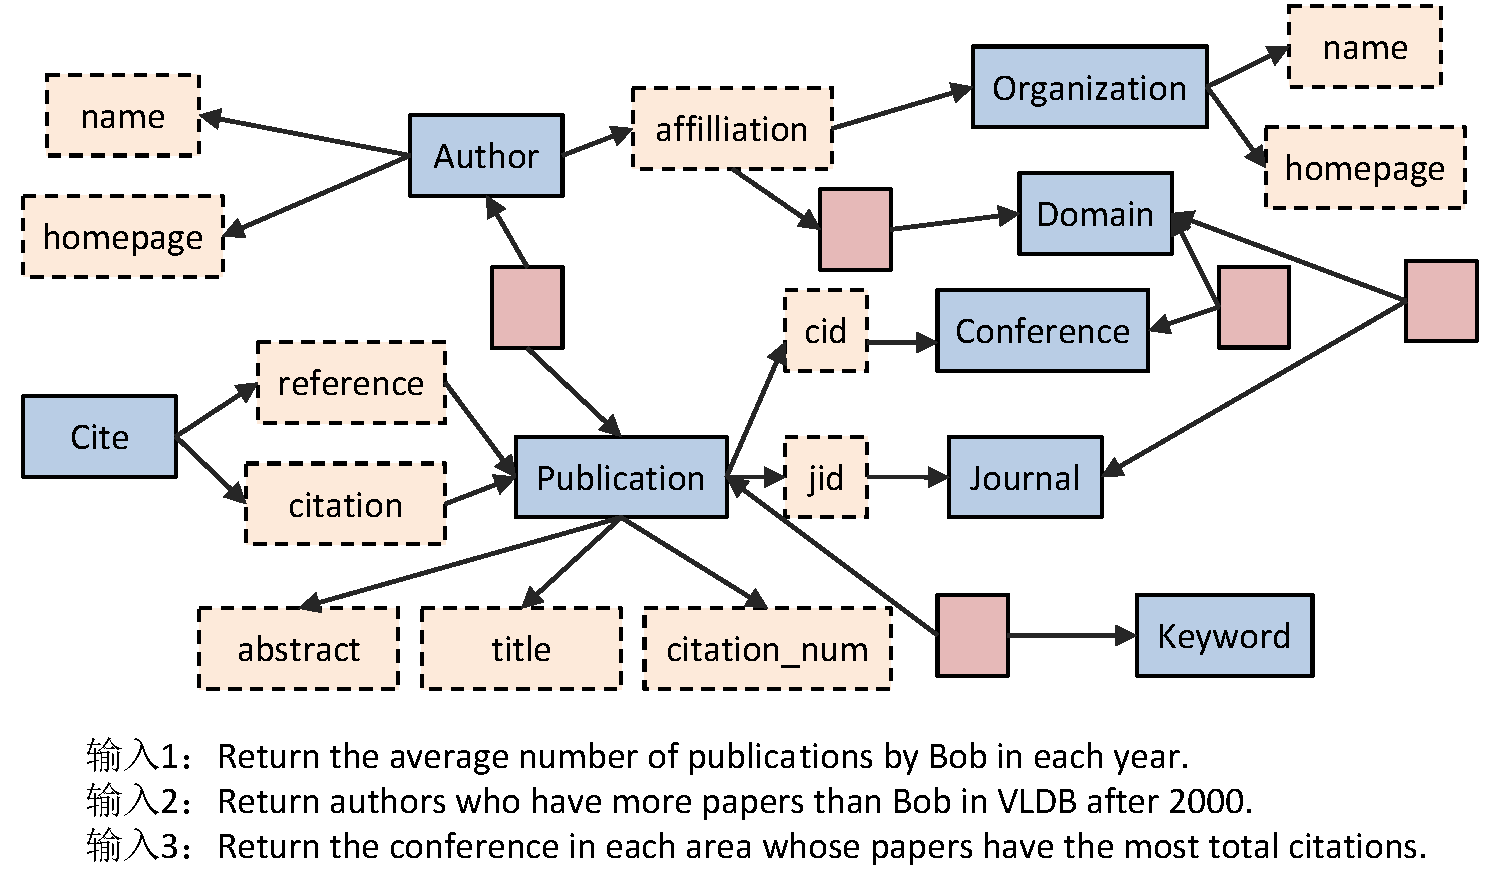
\includegraphics[width=13cm]{example/NLIschema.pdf}
  \bicaption[查询示例及其图模式]
    {查询示例及其图模式}
    {Query Examples and Graph Schema}
  \label{fig:NLIschema}
\end{figure}

需要特别说明的是,一般的搜索引擎提供的方案或者之前的NLIDB的方案所产生的结果通常无法解释。
例如,假设用户的输入是图\ref{fig:NLIschema}中的输入1,使用之前的方案可以得到结果为数字5,而用户无法知道这个答案是否是正确的;
除此之外,由于自然语言的表达十分复杂,用户的输入可能是模棱两可的。
例如,假设用户的输入是图\ref{fig:NLIschema}中的输入1,查询语句中所使用的单词是“publication”,而在业务数据库中,“publication”在数据库中对应的可能是表中的“article”,“journal”等字段。
因此,在基于映射的INL2SQL中,本文并不是直接产生查询的结果,而是向用户解释解析的过程,并通过多轮的交互修复解析中产生的“歧义”问题。

\begin{figure}[!htp]
  \centering
  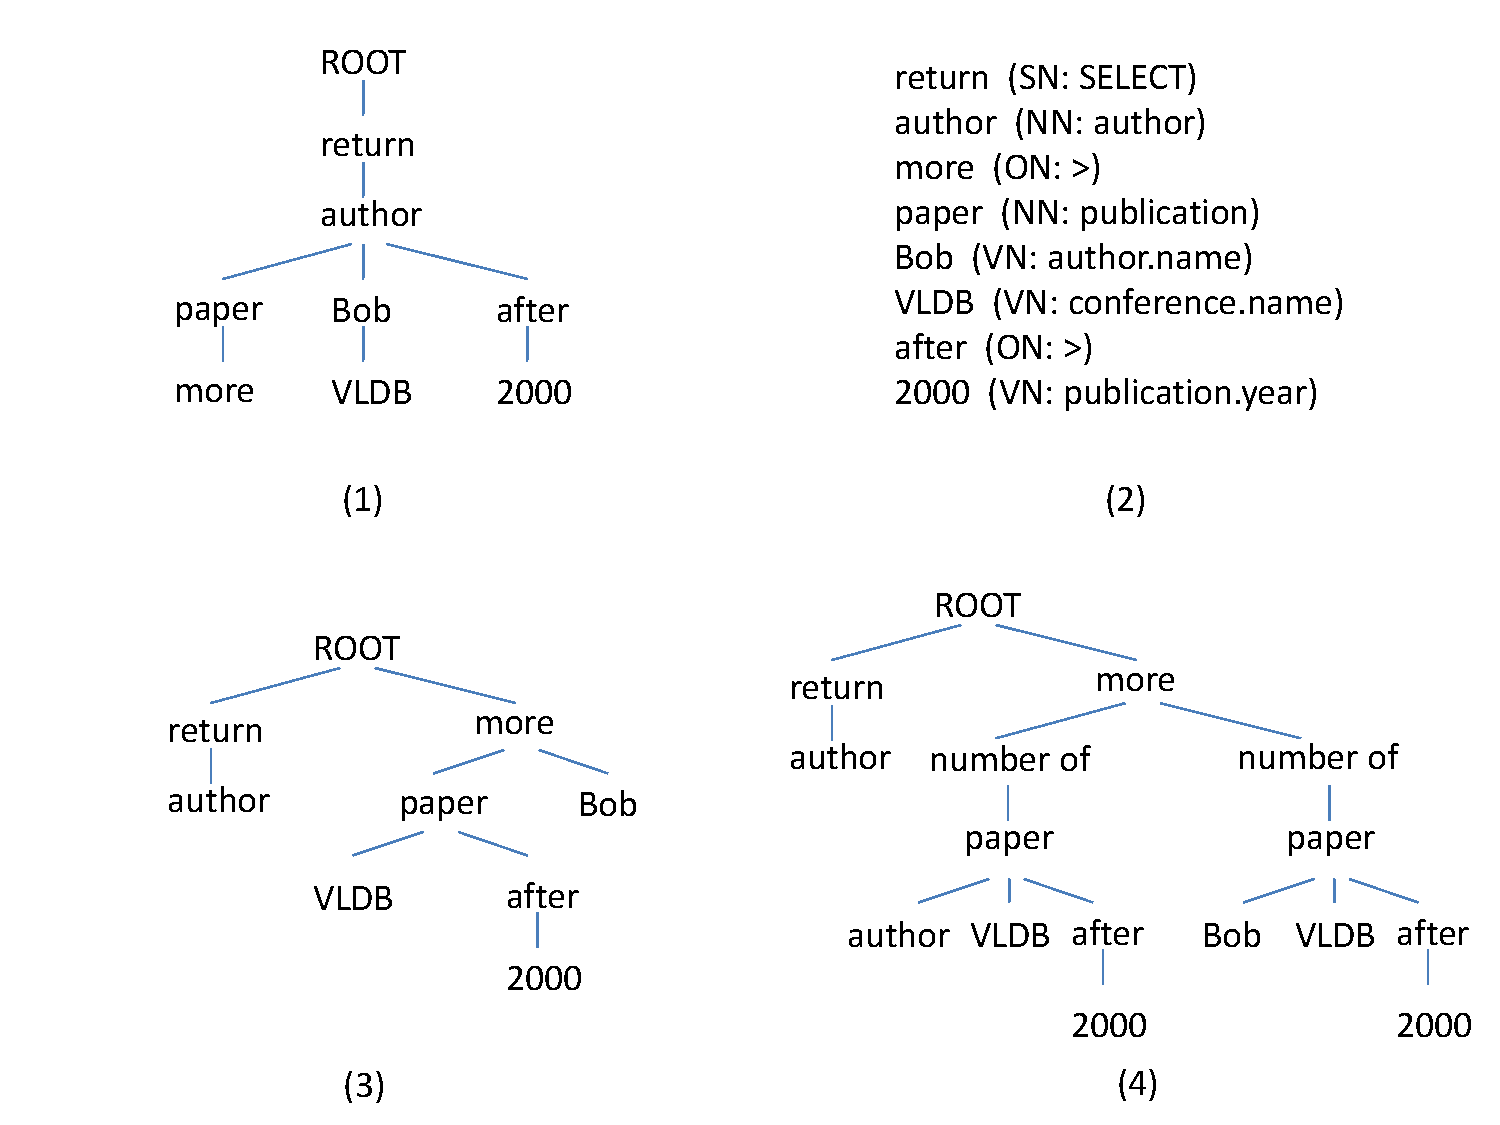
\includegraphics[width=13cm]{example/NLIexample.pdf}
  \bicaption[解析过程示例]
    {解析过程示例}
    {Example of Parsing Process}
  \label{fig:NLIexample}
\end{figure}

在此,先给出基于映射的INL2SQL生成的整个解析过程的示例(如图\ref{fig:NLIexample}所示),再对解决方案中的每个模块进行详细阐述。
第一步,通过依赖解析树生成模块,系统将用户的自然语言查询输入(图\ref{fig:NLIschema}中的输入2)转换为一颗简单的语法解析树(图\ref{fig:NLIexample}(1))。
第二步,解析树节点映射模块为解析树种的每个节点生成一个最佳映射(图\ref{fig:NLIexample}(2)),并通过意图交互模块向用户通知“VLDB”节点在数据库模式中可以映射为“conference”和"journal"而系统选择了“conference”作为其默认映射。
第三步,解析树优化重构模块将根据最佳映射对解析树进行重构和调整,生成k个有效的解析树。同时,意图交互模块会结合自然语言模板将这k个候选的解析树告知用户并让用户进行选择,例如:“return the authors, where the papers of the author in VLDB after 2000 is more than Bob”。被选择的最佳的解析树如图\ref{fig:NLIexample}(3)。
之后,通过插入一些隐藏节点,解析树被实例化为图\ref{fig:NLIexample}(4),与用户的交互为“return the authors, where the number of papers of the author in VLDB after 2000 is more than the number of paper of Bob \underline{in VLDB} \underline{after 2000}"。
若用户需要取消\underline{in VLDB}和\underline{after 2000},系统将继续执行第二步和第三步。
第四步,查询树翻译模块将结合SQL语句的表达式将最终确认的解析树转换为SQL查询语句并返回给用户。

接下来,本文将详细阐述依赖解析树模块、解析树节点映射模块、解析树优化重构模块、查询树翻译器的设计思路和实现细节。

% \subsection{查询机制}
% \label{nli:cxjz}


% \begin{figure}[!htp]
%   \centering
%   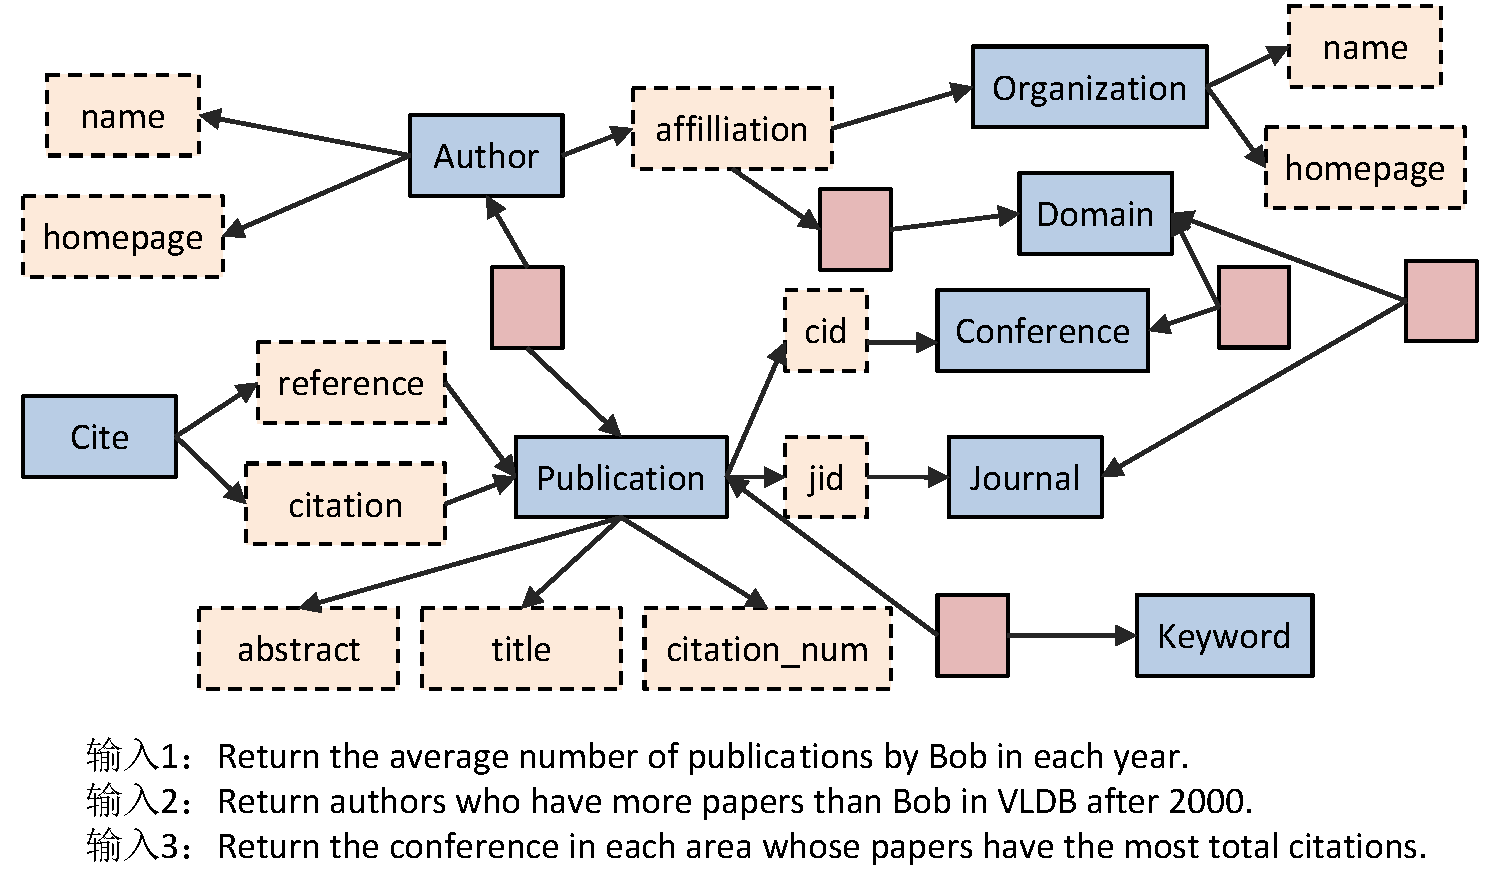
\includegraphics[width=15cm]{example/NLIschema.pdf}
%   \bicaption[示例的解析模式]
%     {示例的解析模式}
%     {write}
%   \label{fig:NLIschema}
% \end{figure}

\subsection{依赖解析树生成}
\label{nli:yljxssc}

本模块将用户输入的自然语言查询解析为解析树,主要内容包含词语的词性标注、关系提取等。

在具体实现过程中,这一模块基于Stanford Parser\cite{de2006generating}实现。
Stanford Parser是斯坦福大学推出的自然语言处理工具,提供依赖解析、命名实体识别、词性标注、情感分析、机器翻译等多种功能。
本模块调用该工具,使用依赖解析的相关接口将自然语言查询解析为依赖解析树。
如图\ref{fig:NLIexample}(1)所示,依赖解析树的每个节点为用户输入的单词或短语,每条边为提取出的单词之间的语义依赖关系。

\subsection{解析树节点映射}
\label{nli:jxsjdys}
本模块将依赖解析树的节点对应的词语,映射到SQL组件上。解析树节点的类型定义如表\ref{nli:jxsjddlx}所示。

% 这一节给出的是一些表格的例子,如表\ref{nli:jxsjddlx}所示。

\begin{table}[!hpb]
  \centering
  \bicaption[解析树节点的类型]
    {解析树节点的类型}
    {Different Types of Nodes}
  \label{nli:jxsjddlx}
  \begin{tabular}{@{}llr@{}} \toprule
    % \multicolumn{2}{c}{Item} \\ \cmidrule(r){1-2}
    节点类型 & 对应的SQL组件\\\midrule
    选择节点(SN) & SELECT\\
    操作符节点(ON) & 一个操作符,如等于(“=”)、小于(“<”)\\
    聚合函数节点(FN) & 一个聚合函数,如AVG、MAX\\
    名字节点(NN) & 业务数据库中的一个数据表的名字,或数据表的一个字段的名字\\
    值节点(VN) & 业务数据库中某字段的一个值\\
    度量节点(QN) & ALL,ANY,EACH\\
    逻辑节点(LN) & AND,OR,NOT\\\bottomrule

    % Animal & Description & Price (\$)\\ \midrule
    % Gnat & per gram & 13.65 \\
    % & each & 0.01 \\
    % Gnu & stuffed & 92.50 \\
    % Emu & stuffed & 33.33 \\
    % Armadillo & frozen & 8.99 \\ \bottomrule
  \end{tabular}
\end{table}
% \footnotetext[1]{这个例子来自\href{http://www.ctan.org/tex-archive/macros/latex/contrib/booktabs/booktabs.pdf}{《Publication quality tables in LATEX》}(booktabs宏包的文档)。这也是一个在表格中使用脚注的例子,请留意与threeparttable实现的效果有何不同。}


其中名字节点和值节点是与当前应用的业务数据库有关,其余五种节点都与业务数据库无关,仅与SQL语法规则相关。
所以,本系统建立了一个五种与业务数据库无关的节点类型与自然语言单词的词典映射。映射过程的实现如下:
对每一个解析树节点对应的单词$n$,分别计算其与业务数据库元数据、存储数据、词典映射中词语v的相似度$Sim_{wup}(n,v)$,$Sim_{gram}(n,v)$的定义如公式\ref{nli:eq1}所示:

%   \begin{equation}
%     \label{eq:res}
%     \ointop_{\gamma}f(z)\,\mathrm{d}z = 2\uppi\mathbf{i}\sum^n_{k=1}\mathrm{I}(\gamma,a_k)\mathrm{Res}(f,a_k)
%   \end{equation}
  \begin{equation}
    \label{nli:eq1}
    % Sim \left ( n ,\right v) = \max\left ( Sim_{wup}\left ( n ,\right v) ,\right Sim_{gram}\left ( n ,\right v))
    Sim(n,v) = \max(Sim_{wup}(n,v),Sim_{gram}(n,v))
\end{equation}

其中$Sim_{wup}(n,v)$为$n$和$v$的WUP相似度\cite{wu1994verb},$Sim_{gram}(n,v)$为$n$和$v$的q-gram的Jaccard相似度的平方根\cite{xiao2011efficient}。
经公式计算,可以得到节点单词$n$与所有SQL组件的相似度;
对相似度进行排序,可以得到前五相似的SQL组件,如果前五相似的SQL组件的相似度$Sim(n,v)$的值差别较大,则直接以相似度最高的SQL组件作为当前单词n的映射,并赋予该组件对应的节点类型;
若前五相似的SQL组件的相似度差别较小,则视作歧义,将候选的SQL组件返回给用户,让用户来进行选择,最后用户选择的结果会作为当前节点的映射。 


\subsection{解析树优化重构}
\label{nli:jxsyhcg}

节点映射完成后,需要对解析树的结构进行重构,保证解析树的结构能有较高的准确性。
由于解析树可能会存在关系解析错误和节点关系缺失,所以这一模块对于解析树的优化重构会分为两个步骤进行,分别为结构调整和隐藏节点插入。

\subsubsection{结构调整}

\begin{table}[!hpb]
  \centering
  \bicaption[合法解析树结构规则]
    {合法解析树结构规则}
    {Grammar of Valid Parse Trees}
  \label{nli:hfjxsjggz}
  \begin{tabular}{@{}llr@{}} \toprule
    % \multicolumn{2}{c}{Item} \\ \cmidrule(r){1-2}
    1  & 	Q -> ( SClause ) ( ComplexCondition ) *\\
    2  & 	SClause -> SELECT + GNP\\
    3  & 	ComplexCondition -> ON + ( leftSubtree * rightSubtree )\\
    4  & 	leftSubtree -> GNP\\
    5  & 	rightSubtree -> GNP | VN | MIN | MAX\\
    6  & 	GNP -> ( FN + GNP ) | NP\\
    7  & 	NP -> NN + ( NN ) * ( Condition ) *\\
    8  & 	condition -> VN | ( ON + VN )\\\bottomrule
  \end{tabular}
\end{table}

在进行结构调整之前,首先定义什么样的树结构是好的、合法的。
本文从两个角度来考虑这个问题:第一点是树结构与经依赖解析器解析后的原始结构的差别有多大;
第二点是树结构是否符合SQL的语法,这一点的评估可以根据表\ref{nli:hfjxsjggz}的定义来确定\cite{li2014constructing}。

表\ref{nli:hfjxsjggz}根据SQL语句的语法,结合了树状结构,定义了能合理的转化为SQL语句的语法树应该满足什么样的规则,这样的语法树在本文中称为查询树。
在表\ref{nli:hfjxsjggz}中,“ + ”代表父子节点的关系,“ * ”代表兄弟节点的关系,上标“ * ”代表可重复出现的兄弟节点,“ | ”代表“或者关系”,表示当前节点可能存在的情况。
% 这是写在算法\ref{algo:sum_100}前面的一段话,在生成的文件里它会出现在算法\ref{algo:sum_100}前面。
\begin{algorithm}
    % \begin{algorithm}[H] % 强制定位
    \caption{解析树结构调整算法}
    \label{nli:jxsjgtzsf}
    \begin{algorithmic}[1] %每行显示行号
    \Ensure 结构调整之后的解析树结果集 % 输出
    % \State $sum \gets 0$
    % \For{$i = 0 \to 100$}
    %     \State $sum \gets sum + i$
    %   \EndFor
    \State $results \gets empty\_set()$
    \State $priorityQueue \gets empty\_priority\_queue()$
    \State $priorityQueue \gets priorityQueue + parseTree$
    % priorityQueue.push(parseTree)
    \State $hash\_table \gets empty\_set()$
    \State $hash\_table \gets hash\_table +hash(parseTree)$
    % hash\_table.add(hash(parseTree))
    \While{$priorityQueue != empty\_priority\_queue()$}
        \State $tree \gets priorityQueue.pop()$
        \State $treeList \gets adjust(tree)$
        \For{$adjustTree in treeList $}
        \If{$hash(adjustTree) not in hash\_table$ \textbf{and} $adjustTree.edit < t$}
            \State $adjustTree.edit \gets tree.edit + 1$
            \State $hash\_table \gets hash\_table + hash(adjustTree)$
            % hash\_table.add(hash(adjustTree))
            \If{$evaluate(adjustTree) >= evaluate(tree)$}
                \State $priorityQueue.add(tree’)$
            \EndIf
            \If{adjustTree is valid}
                \State $results.add(adjustTree)$
            \EndIf
        \EndIf
        \EndFor
    \EndWhile
    \State $results \gets rank(results)$
    \State \Return$results$
    \end{algorithmic}
    \end{algorithm}

算法\ref{nli:jxsjgtzsf}展示了结构调整的算法,算法的基本思想是,建立一个优先级队列,对于当前的解析树,调用adjust()函数(第8行),通过一次移动子树操作,生成在这一次操作后所有可能的结构;
然后记录当前树的哈希值(第12行),防止之后出现重复的树结构;
若当前树结构没有出现过(第10行),且edit值小于一个阈值,则对此树进行下一步操作;
由于移动了一次子树,返回的树的edit属性加一(第11行),这一属性将用来评估生成的树结构与原始结构的差异;
调用evaluate()函数,记录当前结构有多少节点不满足表\ref{nli:hfjxsjggz}设定的规则,不满足规则的节点数将用来评估树结构在语法上的合法性;
综合这两方面评估标准,为树打分,如果分数比之前的树结构要高,则加入优先级队列;
若该树完全符合语法规则,则视为一颗查询树,加入result集合;
之后对优先级队列内的树结构重复以上操作,直到优先级队列为空;最后根据评估分数对result集合排序,将结果返回。

结构调整之后的解析树结果集,将会通过交互式对话器,与用户进行交互,因为结果集中的解析树虽然都符合SQL语法规则,但仍有可能存在与用户意图不同的情况,如SELECT子句中的名字节点和WHERE子句中的名字节点,位置可能会互换,虽然仍然符合SQL语法规则,但与原始查询意图已经有比较大的差别了。
所以,在这里需要再一次应用人机交互机制,让用户来选择结果集中与自己的查询意图比较相似的解析树。交互完成后,筛选出的结果集,会进入下一步——隐藏节点插入。

\subsubsection{隐藏节点插入}

\begin{figure}[!htp]
  \centering
  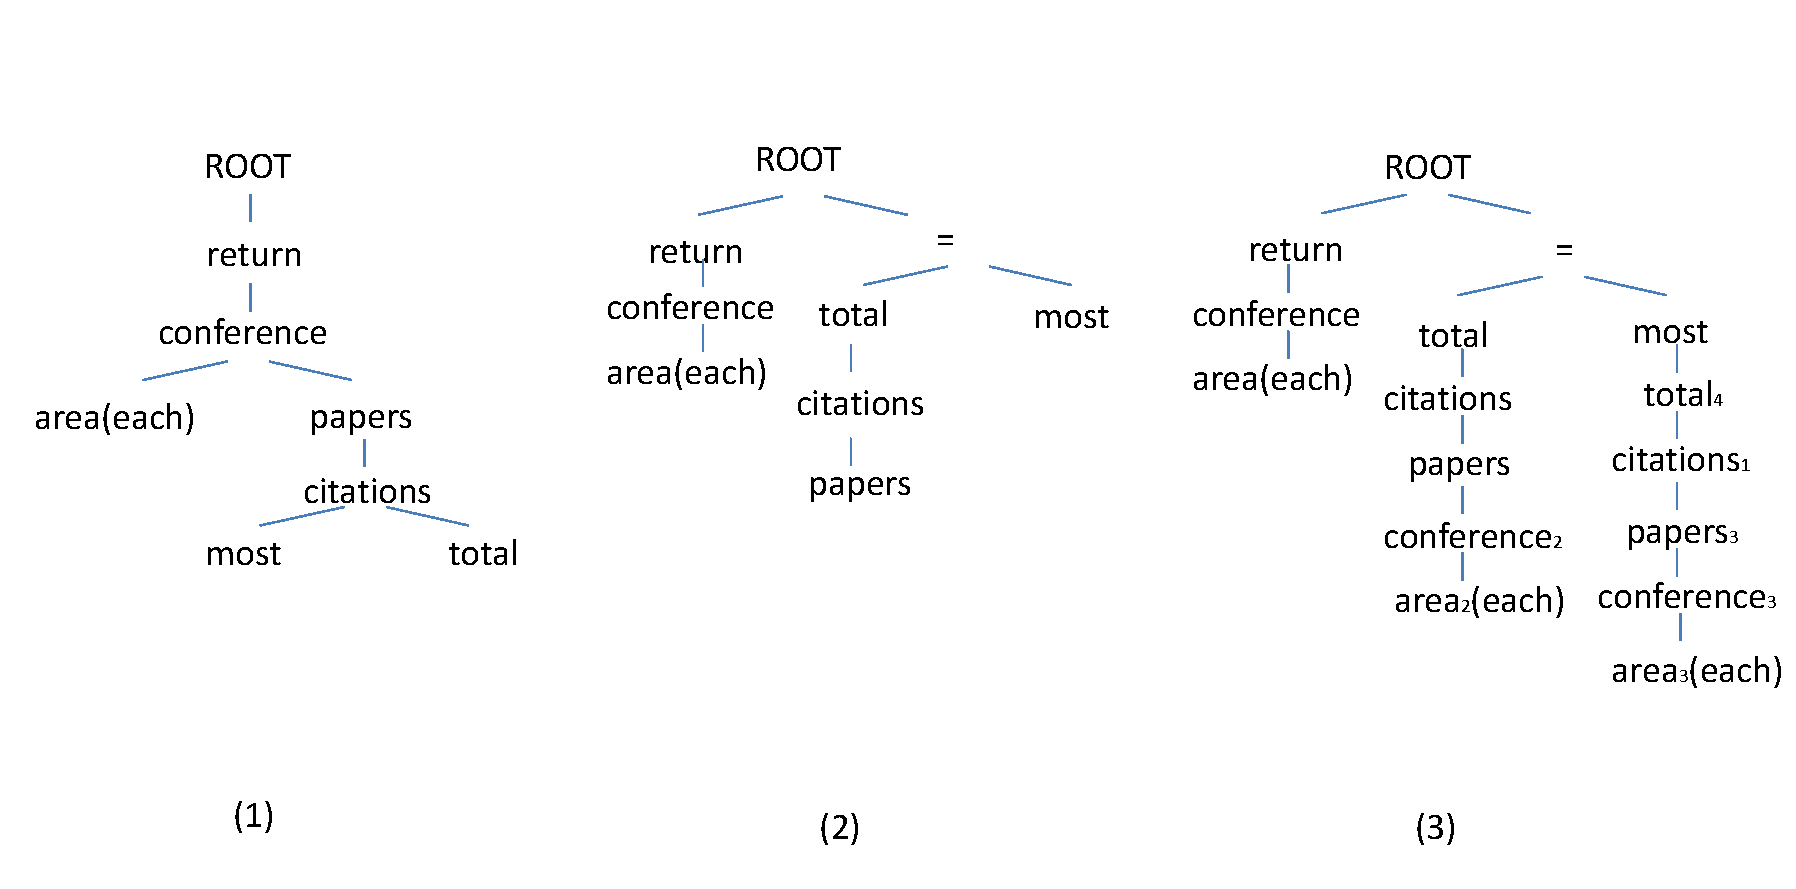
\includegraphics[width=13cm]{example/NLIimplicit.pdf}
  \bicaption[隐藏节点插入过程示例]
    {隐藏节点插入过程示例}
    {Steps of Parsing}
  \label{fig:NLIimplicit}
\end{figure}

结构调整完成后,对经过排序和用户交互筛选后的结果集合,进行隐藏节点插入。
图\ref{fig:NLIimplicit}展示了图\ref{fig:NLIschema}中的输入3从简单的解析树、有效解析树再到隐藏节点插入后的解析树的过程。
在给出隐藏节点插入的方法之前,先给出需要用到的概念定义,即“核心节点”。
核心节点指的是在节点类型为leftSubtree和rightSubtree的情况下(表\ref{nli:hfjxsjggz}),leftSubtree(rightSubtree)的所有子节点中,高度最高的名称节点被称为核心节点。

经过研究,需要进行隐藏节点插入的情况有以下几种:
\begin{enumerate}
    \item 左子树(leftSubtree)与右子树(rightSubtree)的核心节点对应了不同的SQL组件,即认为右子树真正的核心节点在自然语言表达时被省略了\cite{zeng2014breaking};
    这是十分常见的现象,因为人在进行自然语言表达时,对两个值进行比较时,会很自然的省略掉后者的一部分,如“I have more books than yours”这句话,就将最后的“your books”给省略成了“yours”;
    \item 左右子树的约束条件应该一致,如果不一致,则认为右子树一部分约束条件被省略了,如“return authors whose papers published in 2018 more than Jack’s”这句话,过滤条件的左子树有“in 2018”这一约束,而右子树在解析之后没有这一约束,事实上右子树的这一约束被隐藏了,需要作为隐藏节点插入进去;
    \item 某些函数会被省略,如聚合函数“COUNT”,在自然语言表达中经常会被省略,如“I have more books than yours”这句话,“the number of”就被省略了。在树结构中,如果过滤条件的操作符为“more”、“less”等词语,而左右子树的核心节点对应的是非数字类型的SQL组件,那么就认为“COUNT”被省略了,需要作为隐藏节点插入解析树。
\end{enumerate}
% 1)	左子树(leftSubtree)与右子树(rightSubtree)的核心节点对应了不同的SQL组件,即认为右子树真正的核心节点在自然语言表达时被省略了[14];这是十分常见的现象,因为人在进行自然语言表达时,对两个值进行比较时,会很自然的省略掉后者的一部分,如“Ihavemorebooksthanyours”这句话,就将最后的“yourbooks”给省略成了“yours”;
% 2)	左右子树的约束条件应该一致,如果不一致,则认为右子树一部分约束条件被省略了,如“returnauthorswhosepaperspublishedin2018morethanJack’s”这句话,过滤条件的左子树有“in2018”这一约束,而右子树在解析之后没有这一约束,事实上右子树的这一约束被隐藏了,需要作为隐藏节点插入进去;
% 3)	某些函数会被省略,如聚合函数“COUNT”,在自然语言表达中经常会被省略,如“Ihavemorebooksthanyours”这句话,“thenumberof”就被省略了。在树结构中,如果过滤条件的操作符为“more”、“less”等词语,而左右子树的核心节点对应的是非数字类型的SQL组件,那么就认为“COUNT”被省略了,需要作为隐藏节点插入解析树。

进行隐藏节点插入之后,查询树的结构就比较完整了,将会输入下一模块进行翻译。

\subsection{查询树翻译}
\label{nli:cxsfy}
这一阶段的查询树已经在节点映射、树结构、完整性方面都比较可信、合法了,翻译步骤如下:
\begin{enumerate}
    \item 根据表\ref{nli:hfjxsjggz}中的树结构,在SClause子树下的结构为SELECT子句,读取SClause下的名称节点,根据对应的SQL组件(如果SQL组件对应某数据表,该数据表会预定义一个核心字段,如用户的名字、城市的名称,该数据表的核心字段将作为结果返回),填充入SELECT子句,并记录SQL组件对应的数据表,以备FROM子句的生成。
    \item 在ComplexCondition子树下的结构为WHERE子句,分别读取左子树和右子树核心节点对应的SQL组件,记录下SQL组件对应的数据表,并查看左右子树中所有的节点,根据其节点类型,将其翻译为对应的SQL组件,并应用于核心节点;左右子树解析完后,以操作符连接左右子树,将其填充入WHERE子句。
    \item 根据之前记录的相关数据表,生成SQL语句的FROM子句。
    \item 将三部分按照语法连接起来,作为合法的SQL语句返回给用户。
\end{enumerate}

\section{实验与分析}
为了评估基于映射的INL2SQL方法的准确性,本文采用 Classicmodels 和 MAS 数据集进行了实验。
\subsection{评价指标}
INL2SQL的目标是尽可能让使用者使用更加自然的自然语言的方式来生成SQL查询语句,如何评价INL2SQL系统的有效性是其中比较有挑战的问题。
在此背景下,传统的信息检索所使用的指标(如精确度和召回度)不太适用与这个场景。
例如,当生成的SQL语句有效时,精确度为100\%;而当生成的SQL不完全有效时,得到的精确度往往为0\%,这不能很好的显示出系统的有效性。
因此,本文采用的评价指标为准确性,其定义为输入的查询语句经过多轮交互后完美符合用户期望的比例,在最后一次交互时用户确认生成有效时记为正确生成,用户在任意时刻认为SQL生成无效时记为错误生成。
需要说明的时,即使最后生成的SQL语句与标准答案高度一致但用户认为此次生成无效时,本文也会认为是一次错误生成。
因此,该评价指标是更为严格的。

\subsection{数据集}

\begin{figure}[!htp]
    \centering
    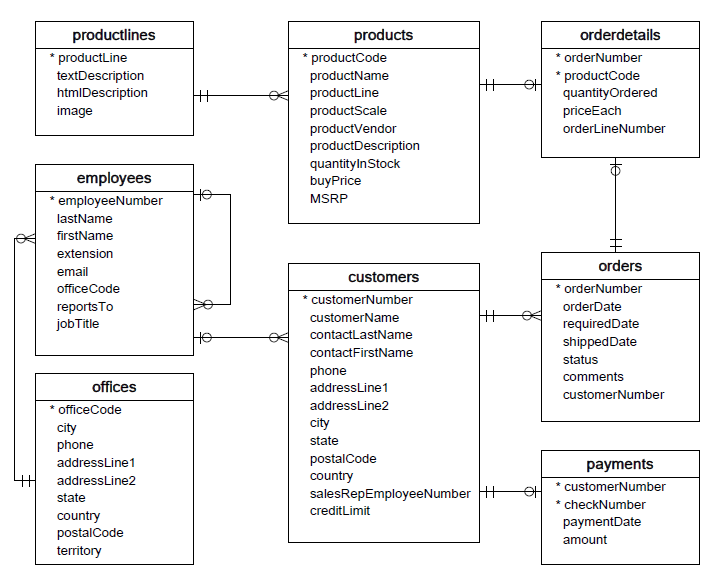
\includegraphics[width=13cm]{example/classicmodel.png}
    \bicaption[Classicmodels数据库的数据库模式图]
      {Classicmodels数据库的数据库模式图}
      {Database Schema of Classicmodels Database}
    \label{fig:NLIclassicmodel}
  \end{figure}

  \begin{table}[!hpb]
    \centering
    \bicaption[MAS数据库数据统计]
      {MAS数据库数据统计}
      {MAS Database Statistics}
    \label{nli:MASsjksjtj}
    \begin{tabular}{|c|c|c|c|} 
      % \toprule
      % \multicolumn{2}{c}{Item} \\ \cmidrule(r){1-2}
      \hline
      表名 & 数据量 & 表名 & 数据量\\
      \hline
      Publica & 2.45M & Author & 1.25M\\
      \hline
      cite & 20.3M & Domain & 24\\
      \hline
      Conference & 2.9K & Journal & 1.1K\\
      \hline
      Organiza & 11K & Keywords & 37K\\
      \hline
      % 简单 & return all the custormers\\
      % 中等 & return all the offices in London\\
      % 困难 & return the city of office that has an employee named Diane\\
      % \bottomrule
    \end{tabular}
  \end{table}


本次实验所使用的业务数据库为MySQL的样例数据库Classicmodels以及MAS(Microsoft Academic Search)数据库,图\ref{fig:NLIclassicmodel}为Classicmodels数据库的数据库模式图,图\ref{fig:NLIschema}和表\ref{nli:MASsjksjtj}为MAS的模式图和数据统计。
实验所使用的自然语言查询数据集根据查询意图的复杂度,分为简单、中等、困难三类。
Classicmodels数据集中的每种类别,提出了20条自然语言查询,共计60条,用来测试模型的有效性。
MAS数据集中的每个类别有100条自然语言查询,共计300条,用于测试模型的准确性。

\begin{table}[!hpb]
  \centering
  \bicaption[自然语言查询实例]
    {自然语言查询实例}
    {Instances of Natural Qanguage Query}
  \label{nli:zryycxsl}
  \begin{tabular}{cc} \toprule
    % \multicolumn{2}{c}{Item} \\ \cmidrule(r){1-2}
    查询语句复杂度 & Classicmodels数据集\\\midrule
    简单 & return all the custormers\\
    中等 & return all the offices in London\\
    困难 & return the city of office that has an employee named Diane\\
    \midrule
    查询语句复杂度 & MAS数据集\\\midrule
    简单 & return all the conferences in database area\\
    中等 & return the number of papers in each database conference\\
    困难 & return the author who has the most publications in database area\\
    \bottomrule
  \end{tabular}
\end{table}
表\ref{nli:zryycxsl}给出了三种类别的自然语言查询示例,上半部分为Classicmodels数据集,下半部分为MAS数据集。

\subsection{实验结果}

\begin{table}[!hpb]
  \centering
  \bicaption[模型生成SQL语句的准确性]
    {模型生成SQL语句的准确性}
    {The Accuracy of Generating SQL Statements}
  \label{nli:mxscsyjdzqx}
  \begin{tabular}{cccc} \toprule
    % \multicolumn{2}{c}{Item} \\ \cmidrule(r){1-2}
    数据集 & 简单 & 中等 & 困难\\
    \midrule
    Classicmodels数据集(无交互)& 65\% & 50\% & 15\% \\
    Classicmodels数据集(有交互)& 100\% & 80\% & 35\% \\
    MAS数据集准确率(无交互) & 63\% & 47\% & 29\% \\
    MAS数据集准确率(有交互) & 100\% & 93\% & 71\% \\
    \bottomrule
  \end{tabular}
\end{table}

首先将所有自然语言查询语句,输入系统,经过各组件的处理,得到系统生成的SQL语句,再判断其是否正确表达了自然语言查询语句的意图。
实验结果如表\ref{nli:mxscsyjdzqx}所示。
实验检验了没有用户交互和有交互的场景下,模型生成SQL语句的准确性。
需要说明的是,无论有无交互,在没有选择合适树结构时,导致解析树结构调整之后有多个候选结果,最后返回结果也会有多个,故只要返回结果中包含正确SQL语句,就视做SQL生成正确。
从模型在Classicmodels数据集上的实验结果来看,模型在有交互的场景下的准确性相较无交互的场景下有较大提升,证明了本文模型的可用性。
从在MAS数据集上的实验结果来看,模型在有交互的情况下在简单、中等、困难的场景下的表现为100\%,93\%,71\%,超过了66.7\%,54.5\%,54.5\%的最高水平\cite{simitsis2008precis}。



\subsection{实验分析}
\begin{enumerate}
    \item 经过如上实验,分别检验了完整模型在有无交互机制的场景下生成SQL语句的准确性。可以看出,交互机制对于模型的准确性有很大的提升;而加入了交互机制后,模型可以比较准确的处理简单和中等复杂度的查询意图,即便是复杂度较高的查询意图,本文提出的模型仍然可以正确生成一部分困难复杂度的SQL语句。在实验过程中,经常出现节点歧义需要映射,如“price”一词可以映射到“products”表中的“buyPrice”,也有可能映射到“orderdetails”表中的“priceEach”。那么对于测试语句“return order details whose price is higher than 50”,如果没有交互机制,对于“price”这个节点的映射就会优先映射到“products”中的“buyPrice”,而实际上应该映射到“orderdetails”表中的“priceEach”。可以看出,交互机制在节点映射这一部分准确率的提升,大大影响了整体模型的准确率。
    \item	在Classicmodels数据集上构造的自然语句查询意图数据集中,简单复杂度的查询意图大体上是返回某数据表中某一字段,中等复杂度的查询意图会添加一些聚合函数和简单过滤条件,困难复杂度的意图会增加更多的聚合函数和跨表查询,总体上来说结构都比较简单。在表\ref{nli:mxscsyjdzqx}所示的结果中,困难复杂度意图的错误生成情况,一部分来源于查询意图对应的SQL语句需要子查询,如“return the customer who has the most orders”。目前的模型还不能很好的处理这一种情况,在解析树语法和翻译过程中都还没考虑子查询的情况,这可能是接下来需要进一步进行的工作,即提升模型的处理能力,使其能处理更复杂的查询意图。
    \item	目前模型基于相似度的节点映射机制仍然有不足之处,如“return the mobile number of custormer whose name is Australian Gift Network”这一查询意图,对于顾客名称“Australian Gift Network”,系统会将其映射为三个不同的节点,导致生成出错。尽管模型对于数据库模式中的一些连接词或短语,如“the number of”、“customer name”,进行了特殊处理,但对于上文所示的这些特殊短语或词语,目前没有较好的方法来进行处理。
    \item	本文自行建立了一个解析树节点类型与自然语言单词的映射词典(表\ref{nli:jxsjddlx}),能处理一些常见的单词与SQL语法的对应关系,如“return”、“in”、“have”、“thenumberof”,但映射关系仍然不足,所以本实验所使用的测试查询意图都需要使用这些比较固定的词语来构建。事实上,自然语言的表达非常多样,如果要增加模型的处理能力,扩充这个映射词典也是非常必要的。
    \item	尽管人机交互机制对于节点映射的准确率有较大提升,但根据观察,立足于目前数据量较小、数据库模式简单的前提下,这一机制能保证映射相似度排名前五的SQL组件包含正确的映射关系;但随着数据库数据量的增加、数据库模式的复杂化,目前节点映射的相似度计算机制,可能无法确保正确的SQL组件能有较高的相似度。
\end{enumerate}

\section{本章小结}
本章提出了交互式自然语言接口生成SQL语句的方法与技术,基本思想是结合自然语言解析技术,使用人机交互的方式指导解析过程,减轻自然语言解析的歧义问题和错误情况,相比于纯自然语言解析技术,大大提升了准确性。
本章针对自然语言生成SQL语句的方法的准确性进行了实验。实验数据为classicmodels数据集和MAS数据集及其对应的自然语言意图数据集,分别包含简单、中等、困难三种复杂度的查询意图。评估了本方法在有无交互机制的场景下的性能,并给出了实验结果。结果发现,本方法能出色地处理简单和中等复杂度的查询意图,能够较好地处理困难复杂度的查询意图,并且交互机制对准确度的提升非常显著。
但本方法存在无法处理子查询、自然语言意图形式比较固定、无法处理特殊词组等问题,需要进一步进行提升和改进。




